% ------------------------------------------------------------------------------
% Android Patterns Checks: uso de Android Lint para verificação de aderências a
% guidelines 
% Autores:
%     Adorilson Bezerra <adorilson@ppgsc.ufrn.br>
% Licença Creative Commons Atribuição 3.0. 
% Você pode usar e alterar este documento, 
% mas deve obrigatoriamente citar a autoria. 
% ------------------------------------------------------------------------------

\documentclass[a4paper,12pt]{report}

% ------------------------------------------------------------------------------
\usepackage[top=3cm,left=3cm,right=2cm,bottom=2cm]{geometry}
\usepackage[utf8]{inputenc}
\usepackage[brazil]{babel}
\usepackage[pdftex]{graphicx}
\usepackage[normalem]{ulem}   % Sublinhar textos
\usepackage{pslatex}          % Usa fontes standard ao invés das fontes do
                              % LaTeX, melhorando a qualidade dos pdfs gerados
\usepackage{verbatim}
\usepackage{pdflscape}
\usepackage{longtable}
% ------------------------------------------------------------------------------

\title
{
    \vspace{1.5cm}
    \begin{table}[h]
    \centering
    \setlength{\arrayrulewidth}{3.5\arrayrulewidth}
        \begin{tabular}{c}
        \hline\\
        \vspace{0.3cm}
        \Huge Android Patterns Checks: uso de Android Lint \\
        \Huge para verificação de aderências a guidelines\\
        \hline
        \end{tabular}
    \end{table}
}
\author
{
    Adorilson Bezerra\\
    \{adorilson@ppgsc.ufrn.br\}
}
\date{\vspace{1.5cm}\today}

% ------------------------------------------------------------------------------
\begin{document}

\maketitle

\pagenumbering{roman}
\tableofcontents
\listoffigures

\pagebreak
\pagenumbering{arabic}

\pagestyle{headings}

\chapter{Introdução}

\section{Motivação}
O mercado de dispositivos móveis tem crescido muito rapidamente nos últimos anos.
Segundo \cite{lecheta}, estudos mostram que hoje em dia mais de 3 bilhões de pessoas
possuem um aparelho celular. Desenvolvedores de aplicações desejam disponibilizar
seus aplicativos para o máximo número de dispositivos. Dispositivos estes que
possuem diversas diferenças entre si, principalmente considerando smartphones e
tablets: tamanho e qualidade de tela, existência ou não de recursos como telefone
GSM, bluetooth, EDGE, 3G, WiFi, câmera, GPS, bússola, e acelerômetro entre outros.

Um dos fatores que influenciam na escolha de um aparelho é o sistema operacional.
O Android é um dos sistemas operacionais mais utilizados no mundo, estando 
disponível em diversos tipos de aparelhos, com as mais variadas configurações.
O que reforça a necessidade de mecanismos para gerenciar as diversas variações entre 
eles.

Dessa forma, é necessário determinarmos os possíveis pontos de variação da plataforma
Android, assim como entender os mecanismos que a plataforma oferece para auxiliar
o gerenciamento dessas variações. 

Com isso, seremos capazes de criar aplicações que possam ser executadas em dispositivos
com características distintas, e que utilizem esses diferentes recursos de forma otimizada.

% ------------------------------------------------------------------------------
\section{Limitação des trabalhos relacionados}
Escrever a limitação de trabalhos relacionados...

\section{Contribuição do trabalho}
Escrever a contribuição dessa trabalho...

\section{Estrutura do trabalho}
Apresetnar a estrutura do trabalho...


% ==============================================================================
\chapter{Plataforma Android}
Nesse capítulo, apresentaremos a arquitetura da plataforma Android, assim como o
ciclo de vida de uma aplicação para essa plataforma.

% ------------------------------------------------------------------------------
\section{O que é a plataforma Android}
Segundo \cite{whatisandroid}, o Android é uma pilha de software para dispositivos
móveis que inclui um sistema operacional, middleware e aplicações chaves. O Android
SDK fornece as ferramentas e API's necessários para o desenvolvimento de aplicações
para a plataforma, utilizando a linguagem de programação Java.

\subsection{Características}
\begin{itemize}
    \item Framework de aplicações: permite o reuso e troca de componentes.
    Os desenvolvedores têm acesso completo à mesma API que é usada pelas aplicações
    do núcleo da plataforma.
    \item Máquina virtual Dalvik: é uma máquina virtual especializada para o uso em
    dispositivos móveis. Aplicações escritas em Java são compiladas em bytecodes para
    essa máquina virtual, e não uma máquina virtual Java.
    \item Navegador integrado: navegador baseado no motor {\it open source} WebKit
    \item Otimizações gráficas: possibilitadas por uma biblioteca gráfica 2D 
    personalizada; gráficos 3D baseadas na especificação OpenGL ES 1.0 (acelaração
    por hardware opcional)
    \item SQLite: para armazenamento de dados estruturados
    \item Suporte para multimídia: suporte para os formatos mais comuns de 
    áudio, vídeo e imagem (MPEG4, H.264, MP3, AAC, AMR, JPG, PNG, GIF)
    \item Rico ambiente de desenvolvimento: incluindo um emulador de dispositivo,
    ferramentas para depuração, {\it profiling} de memória e perfomance, e um {\it plugin}
    para o Eclipe IDE
    \item Alguns recursos dependentes do dispositivo
        \begin{itemize}
            \item Telefonia GSM 
            \item Bluetooth, EDGE, 3G, e WiFi
            \item Camera, GPS, bússola, e acelerômetro
        \end{itemize}
\end{itemize}

\subsection{Arquitetura da plataforma}

A figura \ref{system-architecture} mostra os principais componentes do sistema 
operacional Android. Cada seção é descrita abaixo.

\begin{figure}[h]
    \centering
    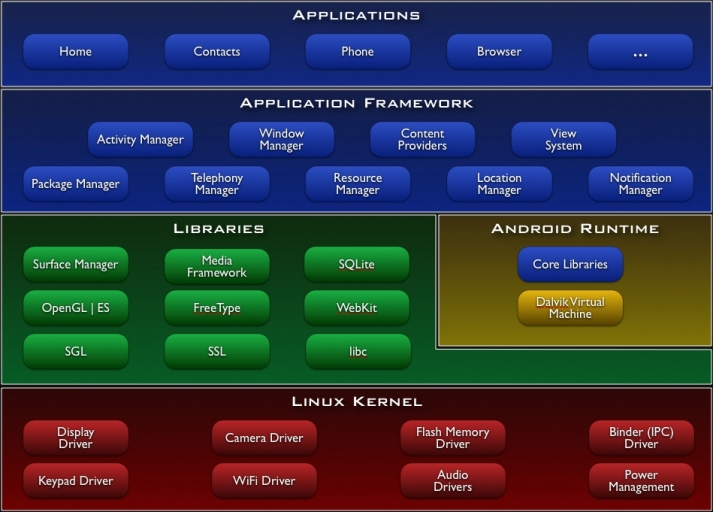
\includegraphics[width=10cm]{img/system-architecture.jpg}
    \caption{Arquitetura da plataforma Android}
    \label{system-architecture}
\end{figure}

\subsubsection{Application}
Android será distribuido com um conjuto de aplicações centrais, incluindo um cliente
de e-mail, programa de SMS, calendário, mapas, navegador, entre outros. Todas as 
aplicações são escritas em Java.

\subsubsection{Application Framework}
Fornecendo uma plataforma de desenvolvimento aberta, Android permite aos desenvolvedores
criarem aplicações extremamente ricas e inovadores. Desenvolvedores são livres para
tirar vantagem do hardware dos dispositivos, acessar informações de localização, 
executar serviços em backgrounds, definir alarmes e notificações para a barra de 
status etc.

Desenvolvedores tem total acesso às mesmas API's do framework usadas pelas aplicações 
do núcleo. A arquitetura da aplicação é projetada para simplificar o reuso de componentes;
qualquer aplicação pode publicar suas funcionalidades e qualquer outra aplicação pode 
fazer uso dessas (sujeito às restrições de segurança impostas pelo framework). Esse mesmo
mecanismo permite que componentes sejam substituídos pelo usuário.

Os principais componentes do Application Framework são:
\begin{itemize}
\sloppy % evita que em linhas muito longas o espaço entre as palavras seja
        % aumentado
    \item System View: uma 'view' representa um widget que aparece na tela
    \item Content Providers: permite que aplicações possam acessar dados de outras 
    aplicações, ou compartilhar seus dados com outras
    \item Resource Manager: fornece acesso para recursos que não são código, como 
    strings de localização, gráficos e arquivos de layout
    \item Notification Manager: permite que as aplicações exibam alertas customizados 
    na barra de status
    \item Activity Manager: gerencia o ciclo de vida das aplicações e fornece um 
    mecanismo comum de navegação
\fussy % dual do \sloppy
\end{itemize}

\subsubsection{Libraries}
Android inclui um conjunto de bibliotecas C/C++ usada por vários componentes do 
sistema. Esses recursos são expostos para os desenvolvedores através do "application 
framework". Algumas das principais bibliotecas são listadas a seguir:

\begin{itemize}
    \item System C library - implementação da bibliotec padrão C (libc), otimizado
    para dispositivos embarcados baseados em Linux
    \item Media Libraries - as bibliotecas suportam a maioria dos formatos mais 
    populares de audio, video e imagem, incluindo MPEG4, H.264, MP3, AAC, AMR, 
    JPG, e PNG
    \item Surface Manager - gerencia o acesso o subsistema do display e composição 
    suave de camadas 2D e 3D para múltiplos dispositivos
    \item LibWebCore - um moderno mecanismo para navegador web que possibilita tanto o 
    navegador do Android quanto um visualizador web embutido
    \item SGL - o mecanismo para gráficos 2D subjacente
    \item 3D libraries - uma implementação baseada na API OpenGL ES 1.0; as bibliotecas
    podem tanto usar a aceleração 3D por hardware (quando disponível), quanto
    a renderação 3D otimizada por software, já incluida.
    \item FreeType - renderização de fonte vetorial e bitmap
    \item SQLite - um poderoso e leve mecanismos de banco de dados relacional, 
    disponível para todas as apliações
\end{itemize}

\subsubsection{Android Runtime}

Android inclui um conjunto de bibliotecas básicas que provê a maioria das funcionalidades
disponíveis na biblioteca padrão da linguagem de programação Java.

Cada aplicação Android executa em seu próprio processo, com sua própria instância 
da máquina virtual Dalvik. Dalvik foi escrita de forma a permitir que um dispositivo
execute multiplas MV's eficientemente. A MV Dalvik executa arquivos no formato de 
Executáveis Dalvik (.dex) que é otimizado para usar o mínimo de memória possível. 
A MV é baseado em registradores, e executa classes compiladas por um compilador Java 
que transforma essas classes no formato .dex com a ferramenta "dx".

\subsubsection{Linux Kernel}

Android depende do Linux para serviços do núcleo do sistema como segurança, gerência
de memória, gerência de processos, pilha de rede e modelo de drivers. O núcleo também
atua como uma camada abstrata entre o hardware e o resto da pilha de sofware.

\subsection{Visão geral sobre as aplicações Android}

Aplicações Android são escritas na linguagem de programação Java. O Android SDK
compila o código - juntamente com seus dados e demais arquivos - em um pacote 
Android, um arquivo com a extensão .apk. É este arquivo que será instalado nos 
dispositivos.

Uma aplicação pode ter quatro tipos de componentes:
\begin{itemize}
    \item Activity: representa uma tela única na interface com o usuário, e podem 
    ser traduzidas para o português como atividades. As atividades
    de uma aplicação são independentes uma das outras, o que possibilita que outra aplicação 
    abra uma atividade (desde de que tenha as permissões necessárias), sem que seja
    necessário abrir a aplicação desta atividade
    Cada atividade é implementada como uma subclasse de Activity. E a definição 
    completa está em \cite{activity}
    \item Service: é um componente que executa em background, sem interface com 
    usuário. Outro componente, como uma atividade, pode iniciar o serviço e deixá-lo 
    em execução ou interagir com ele. Um serviço é implementado como uma subclasse de 
    Service. E a definição completa está em \cite{service}
    \item Content providers: gerencia um conjunto de dados compartilhados da aplicação. 
    Através deste componente, outras aplicações podem consultar ou mesmo modificar 
    dados (se for permitido). Um provedor de conteúdo é implementado como uma subclasse 
    de ContentProvider e deve implementar um conjunto padrão de API's que permite 
    às outras aplicações realizarem as transações. Um detalhamento sobre os provedores
    de conteúdo está em \cite{providers}
    \item Broadcast receivers: é um componente que responde a mensagens enviada ao 
    sistema operacional. Essas mensagens podem ser originadas do próprio sistema, 
    como um alerta de do nível de bateria, por exemplo, ou podem ser enviada por 
    aplicações. Dessa forma, podem ser úteis para fazer a integração entre aplicações.
    Um "broadcast receiver" é implementado como uma subclasse de BroadcastReceiver.
\end{itemize}

Um característica única em sistemas Android é que qualquer aplicação pode iniciar 
um componente de uma outra aplicação. Por exemplo, se você quer enviar alguma mensagem
para o Twitter, provavelmente irá utilizar uma outra aplicação que já faz isso, em vez
de desenvolver uma atividade dentro da sua própria aplicação. Você não precisará 
nem mesmo incorporar ou linkar o código do aplicação do Twitter. Em vez disso, você
simplesmente inicia a aplicação que enviará a mensagem e depois retornará para a sua 
aplicação. Para o usuário, irá parecer que o cliente do Twitter é parte da sua aplicação.

Como cada aplicação é executa em um processo separado, com permissões que restrigem 
o acesso de outras aplicações, sua aplicação não ativa diretamente um componente de 
outra aplicação. O sistema Android é que faz isso. Assim, para ativar um componente 
em outra aplicação, você deve enviar uma mensagem para o sistema que determina sua 
intenção de iniciar um componente em particular. Então, o sistema ativa o componente 
para você.

Essa flexibilidade é possível graças ao ciclo de vida das atividades, descrito na 
seção seguinte.

\subsubsection{Ciclo de vida de uma atividade}

Diferentemente de aplicações em outros sistemas, aplicações Android não possuem 
um único ponto de entrada. Não existe uma função main(), comum na classe principal 
das aplicações Java. O ciclo de vida de uma atividade é apresentada na Figura
\ref{Activity_lifecycle}

\begin{figure}[h]
    \centering
    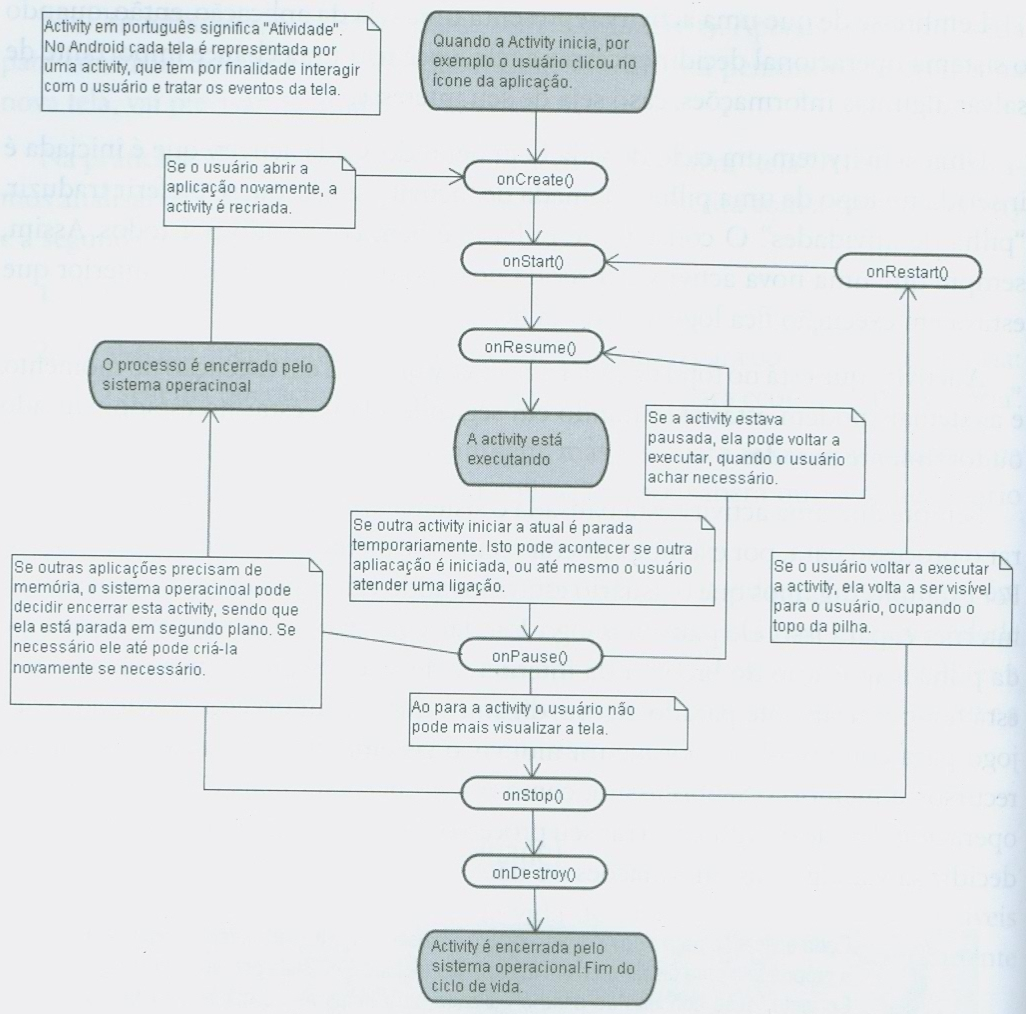
\includegraphics[width=10cm]{img/android_lecheta}
    \caption[Ciclo de vida de uma activity]{Ciclo de vida de uma activity (Fonte: \cite{lecheta})}
    \label{Activity_lifecycle}
\end{figure}

Todos os métodos apresentados na Figura \ref{Activity_lifecycle} são métodos 
da classe Activity, que deverão ser sobrescritos pelas aplicações, e a chamada a
esses métodos ficara a cargo do sistema operacional.

Além desses métodos há um outro importante método automaticamente executado e de 
grande importância do que diz respeito a salvar o estado atual da aplicação: 
{\it onSaveInstanceState(Bundle)}. Este método é executado antes da atividade entrar em 
background, permitindo que seja salvo estado dinâmico em um objeto {\it Bundle}, para depois 
ser recuperado em {\it onCreate(Bundle)}, se a atividade precisa ser recriada. No entanto,
em relação a dados persistentes é necessário que eles sejam salvos no método {\it onPause()}, 
já que o {\it onSaveInstanceState(Bundle)} não faz parte do ciclo de vida, não sendo chamado 
em todas as situações.

% ..............................................................................
\section{Pontos de variações em dispositivos com Android}

Nessa seção, apresentaremos os pontos de variação em dispositivos com Android,
quando possível apresentaremos um exemplo com a aplicação Froid, ou trecho diversos.

\subsection{Versão da API}

A primeira versão da API do Android foi disponibilizada em outubro de 2008. De lá 
para cá, ele vem passando por diversas modificações, sendo a maioria deles 
introdução ou substituições de funcionalidades. Como partes da API são autualizadas, 
as partes antigas são marcadas como obsoletas e não removidas, assim aplicações feitas
com versões antigas da API continuarão funcionando nas mais recentes.

As versões da API são identificadas por um valor inteiro único chamado de {\it API Level},
distribuidas juntamente com as versões da plataforma Android. A Figura \ref{api_level} 
apresenta a relação entre versão da plataforma e {\it API Level}, além da distribuição.

\begin{figure}[h]
    \centering
    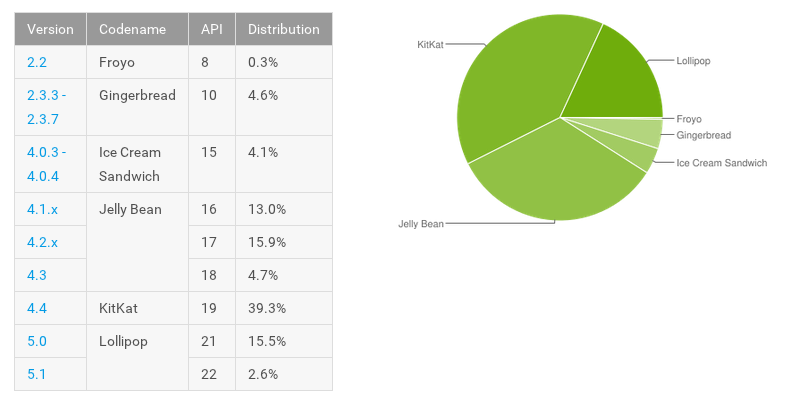
\includegraphics[width=15cm]{img/api_level}
    \caption[Distribuição da versão da plataforma e API Level]{Distribuição da versão
    da plataforma e API Level (Fonte: \cite{dashboards}) }
    \label{api_level}
\end{figure}

\subsection{Tamanhos e densidade das telas}

O Android executa em uma grande variedade de dispositivos, com diferentes tamanhos
 de telas e densidades. Para facilitar o projeto de interface para diferentes 
 configurações, a plataforma divide os atuais intervalos de tamanhos de telas e
 densidades em grupos, conforme abaixo:
\begin{itemize}
    \item Tamanhos de tela: small, normal, large, e xlarge
    \item Densidades: ldpi (low), mdpi (medium), hdpi (high), e xhdpi (extra high)
\end{itemize}
 
A Figura \ref{intervalos_telas} ilustra como os diferentes tamanhos de telas 
(em polegadas) e 
densidades (em dpi) são categorizados nesses diferentes grupos.

\begin{figure}[h]
    \centering
    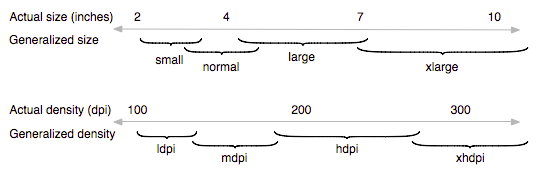
\includegraphics[width=15cm]{img/intervalos_telas}
    \caption[Relação entre tamanhos de telas e densidades e seus respectivos grupos]{Relação entre tamanhos de telas e densidades e seus respectivos grupos 
        (Fonte: \cite{sup_multi_screens}) }
    \label{intervalos_telas}
\end{figure}

\subsection{Versão da OpenGL ES}

O Android oferece suporte para gráficos otimizados através de uma biblioteca 2D 
customizada. Quando suportado pelo hardware do dispositivo, gráficos 3D serão 
providos pela biblioteca OpenGL ES. A Figura \ref{distribuicao_opengl} apresenta 
a distribuição atual de versões dessa biblioteca encontradas nos aparelhos.

\begin{figure}[h]
    \centering
    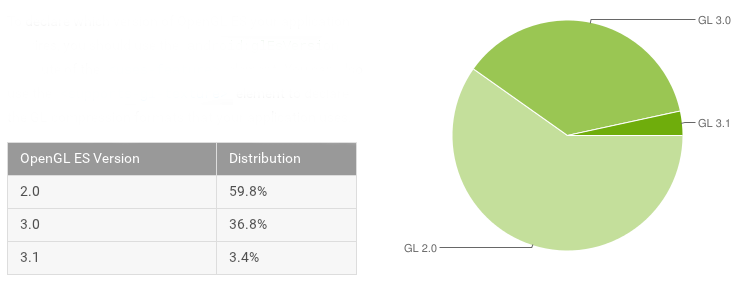
\includegraphics[width=15cm]{img/opengl}
    \caption[Distribuição atual da OpenGL ES]{Distribuição atual da OpenGL ES (Fonte: \cite{dashboards})}
    \label{distribuicao_opengl}
\end{figure}

\subsection{Hardware e sensores do dispositivo}

Android oferece suporte para diversos tipos de sensores e hardware presentes nos 
dispositivos. Contudo, nem todos os dispositivos terão todos os tipos de sensores.
Incluem-se aqui, os mecanismos de interação do usuário com o aparelho.
Sensores e hardware que poderão ou não estar presentes nos dispositivos incluem:
\begin{itemize}
    \item Acelerômetro
    \item Câmera
    \item Sensor de luminosidade
    \item Bluetooth
    \item Wifi
    \item Live wallpaper
    \item GPS
    \item Microfone
    \item Sensor de proximidade
    \item Telefone VoIP baseado em SIP
    \item Telefonia CDMA e/ou GSM
    \item USB
    \item Mecanismos de interação
    \begin{itemize}
        \item Tela sensível a toque e/ou multitoque
        \item Teclado físico
        \item Trackball
        \item Botões de navegação (five-way navigation pad)
    \end{itemize}
\end{itemize}

\subsection{Línguas internacionais}
Os textos das mensagens no sistema operacional costumam estar no idioma nativo do usuário.
É desejável que os textos das aplicações também estejam nesse mesmo idioma, e que 
isso seja possível de forma transparente para o usuário.


\chapter{Trabalho proposto}
\label{trabalho_proposto}
A documentação oficial do Android dispõe de instruções e exemplos sobre como 
preparar uma aplicação a fim de fornecer suporte para as variabilidades acima. 
No entanto, não existe uma ferramenta oficialmente indicada para garantir ou guiar 
esse desenvolvimento, ainda que o Android Lint possa auxiliar de alguma forma essa 
tarefa. Android Lint \cite{lint} faz uso de análise sintática para verificar erros comuns 
em aplicações. Esse trabalho propõe o uso de Android Lint para guiar o desenvolvimento 
de aplicações aderentes aos padrões e boas práticas de desenvolvimento na plataforma Android.

\section{Objetivo geral}
Avaliar o uso de Android Lint para guiar o desenvolvimento de aplicações que seguem 
os padrões e boas práticas de desenvolvimento na plataforma Android

\section{Objetivos específicos}

\begin{itemize}
  \item{Mapear os checks padrões do Android Lint relacionados ao objetivo geral acima}
  \item{Entender como funciona o mecanismo de escrita de novos checks}
  \item{Escrever novos checks para padrões não suportados}
  \item{Aplicar esses checks em projetos}
\end{itemize}

\chapter{Android Lint}
\label{android_lint}
\section{Visão geral}

Android Lint é uma ferramenta oficial disponibilizada pela Google no Android 
Development Toolkit que analisa o código-fonte de projetos Android em busca de 
potenciais erros. Está disponível tanto como uma ferramenta de linha de comando, 
quanto integrado com IDEs, como o Android Studio. Exemplos de erros analisados incluem:

\begin{itemize}
  \item{Traduções incompletas (e traduções não utilizadas)}
  \item{Problemas de performance de layout}
  \item{Recursos (arquivos de imagens e sons, por exemplo) não-utilizados}
  \item{Problemas de internacionalização e acessibilidade}
  \item{Problemas relacionadas a ícones}
  \item{Problemas de usabilidades}
  \item{Erros no arquivo de manifesto, um elemento central no mecanismo de variabilidade
  da plataforma Android \cite{mechanisms}}
\end{itemize}

Atualmente, o Android Lint possui cerca de 190 regras, que agrupam os erros em 
diversos graus de severidade e categorias. Os graus de severidade são 5, que vão 
de apenas informativos, onde não necessariamente é um erro mas que algo no código 
deve ser analisado, até fatal, em que existe um erro crítico no projeto, a ponto 
de falhar a criação do arquivo APK. Quanto às categorias podemos encontrar segurança, 
acessibilidade, internacionalização, usabilidade entre outras. Analisando essa 190 
regras previamente definidas, podemos relacionar cerca de 70 com algum tipo de 
variabilidade ou padrão definido pela plataforma. Como exemplo, podemos citar as 
regras "ButtonOrder", que verifica se a ordem dos botões na interface estão de 
acordo com o padrão de design sugerido pela documentação oficial e "NewApi", 
relacionado a variabilidade de versões da API, que aponta chamadas de métodos 
não-disponíveis em todas as versões da API para qual a aplicação foi desenvolvimento 
(de acordo com a versão mínima específica no arquivo de manifesto). O apêndice 
\ref{apd_cheks_uteis} apresenta uma lista completa dessas regras. 

Para que o Android Lint aplique a analise de uma regra é necessário definir quais 
regras deverão ser utilizadas, o que pode ser feito no arquivo {\it build.gradle} do 
projeto na seção {\it lintoptions}, conforme mostra figura \ref{lintoptions}:

\begin{figure}[h]
    \centering
    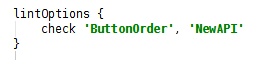
\includegraphics[width=5cm]{img/lintoptions.png}
    \caption{Trecho do arquivo build.gladle, indicando que as regras ButtonOrder e 
    NewApi devem ser executadas}
    \label{lintoptions}
\end{figure}

\section{Criação de novas regras}

Quando são necessárias regras não definidas pelo Lint, novas regras podem ser criadas. 
No entanto, devemos observar que a API do Lint ainda não está estável. Assim, mudanças 
deverão ser necessárias no futuro. Além disso, não existe uma documentação adequada 
dessa API, sendo necessária a leitura do código-fonte tanto da API quanto das regras 
pré-definidas.

Para criar uma nova regra, precisamos fazer a distinção entre “issue” e “detector”. 
“Issue” é um tipo de problema que iremos localizar e mostrar para o desenvolvedor. 
O responsável por fazer essa busca e detecção é um “Detector”.

O tipo de artefato do projeto relacionado ao Issue e que será analisado pelo 
Detector é denominado escopo, que pode ser: arquivos de recursos, código-fonte Java, 
arquivos .class, arquivos de configuração do Proguard e arquivo de manifesto. Quando 
um Issue é criado, seu escopo é definido a partir da classe “Scope”. Por exemplo, 
um Issue relacionado a problemas no arquivo de manifesto tem seu escopo definido 
com Scope.MANIFEST. Esse escopo também terá impacto em quais interfaces um detector 
deverá implementar.

De acordo com a análise necessária, detectors deverão implementar uma ou mais das 
seguintes interfaces: Detector.XmlScanner, Detector.JavaScanner, Detector.ClassScanner. 
Por exemplo, para um detector com escopo para o arquivo de manifesto, deverá implementar 
a interface XmlScanner. E então deveremos implementar o método “visitDocument”, que será 
chamado uma vez para cada arquivo XML, e irá retorno o DOM do XML, que poderá ser utilizado 
para a análise necessária. Contudo, muitas vezes estamos interessados em um tag ou um atributo 
em particular, ou em um conjunto deles. Nesses casos, podemos implementar os métodos 
“getApplicableElements” e/ou “getApplicableAttributes”, que retornam uma lista de strings 
com os nomes das tags ou atributos. Então, implementamos os métodos “visitElement” e/ou 
“visitAttribute”, que serão chamados para cada item das listas retornadas pelos métodos 
citados anteriormente.

Para analisar código-fonte Java, deve-se implementar a interface JavaScanner, da 
qual alguns métodos deverão ser implementados. Entre eles o “createJavaVisitor”, 
que deverá retornar um objeto AstVisitor do projeto Lombok\footnote{https://projectlombok.org/}, 
utilizado pelo Lint para representar ASTs. Também existem alguns métodos para facilitar 
a analise, como o “getApplicableNodeTypes” que especifica tipos de nós a serem analisados 
e “getApplicableMethods”, onde pode ser definido um conjunto de métodos da aplicação
em que estamos interessados.

Já para analise de bytecode a interface ClassScanner é que deverá ser implementada. 
Lint usa a biblioteca ASM\footnote{http://asm.ow2.org/} para processar arquivos .class, que percorre os arquivos 
e produz um objeto ClassNode, que é então passado para cada ClassScanner. Os detectors 
poderão usar esses ClassNodes para analisar o bytecode conforme a necessidade.

\subsection{Reportando erros}
O Lint fornece uma infraestrutura simplificada para reportar os problemas encontrados. 
Basta chamar o método report() no objeto context (que é passado para cada método do detector.). 
Além do problema (Issue) em si, também pode ser fornecido uma localização, um “escopo do nó”, 
e uma mensagem. A localização é o ponto onde o erro ocorreu, o local no DOM se for um XML ou 
o nó da árvore AST se for um código-fonte Java, que irá permitir saber o local exato do arquivo 
onde ocorreu o erro. O “escopo do nó” é o nó AST/XML mais próximo em volta do local do erro. 
Usualmente é o mesmo nó de onde foi criado a localização.


\chapter{Verificação de aderências a guideline}

A plataforma Android suporta uma grande variedades de telas e o sistema redesenha
as interfaces das aplicações de forma a preencher cada uma delas. Tipicamente, 
tudo que o desenvolvedor precisa fazer é projetar a interface para ser flexível 
e otimizar alguns elementos para telas diferentes fornecendo recursos alternativos, 
como layouts alternativos que reposicionam e/ou redefinem dimensões de alguns 
elementos. A fim de facilitar esse trabalho, no Android 3.0 (API Level 11) foi 
introduzida uma nova API: Fragments. Fragmentos permitem separar partes de uma 
interface em componentes isolados, que poderão ser combinados para criar interfaces 
com múltiplos painéis para um tablet ou “activities” separadas para um handset. 
Android 3.0 também introduziu outra API: ActionBar. ActionBar fornece um componente 
no topo da tela para identificar a aplicação e provê ações do usuário e navegação.

A documentação oficial da plataforma fornece guidelines para ajudar desenvolvedores
nessa tarefa de otimizar as aplicações para tablets e handsets\footnote{Disponível 
em http://developer.android.com/guide/practices/tablets-and-handsets.html\#Guidelines}:

\begin{itemize}
    \item{Construir a aplicação baseada em fragmentos que possam ser reutilizados 
    em diferentes combinações;}
    \item{Utilizar ActionBar, mas seguir as melhores práticas e certificar-se que 
    o design da aplicação é flexível o suficiente para o sistema ajustar o layout 
    da action bar baseada no tamanho da tela;}
    \item{Implementar layouts flexíveis.}
\end{itemize}

Neste trabalho, apresentamos uma proposta para automatizar a verificação dos dois 
primeiros itens desse guia. Quanto ao terceiro item, usar fragmentos é parte da
implementação de layouts flexíveis.

\section{Uso da API Fragments}
\label{uso_fragments}
Para a nossa abordagem, definimos que os seguintes items devem ser verificados: 
\begin{itemize}
    \item{As activities deverão ser um “container” de fragmentos;}
    \item{A activity deve, de fato, estar sendo composta por fragmentos}
\end{itemize}


A partir da API Level 11, a classe {\it Activity} já suporta nativamente ser composta
por fragmentos. No entanto, na nossa abordagem iremos considerar que as activies
da aplicação deverão extender, de forma direta ou indireta, da classe FragmentActivity,
do pacote de compatibilidade V4. Assim, também garantiremos que a aplicação dará
suporte para aparelhos com versão mais antigas da API.

Para essa primeira verificação foi definido o Issue MainActivityIsFragmentActivity,
conforme figura \ref{mainactIsFragAct}.

\begin{figure}[h]
    \centering
    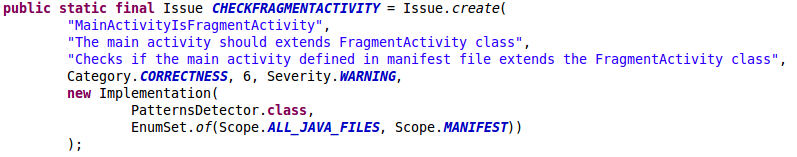
\includegraphics[width=15cm]{img/mainactIsFragAct.png}
    \caption{Definição do issue MainActivityIsFragmentActivity}
    \label{mainactIsFragAct}
\end{figure}

Caso o detector verifique que a activity não esteja fazendo a herança esperada, 
irá reportar, conforme figura \ref{activity_deve_ser_container}

\begin{figure}[h]
    \centering
    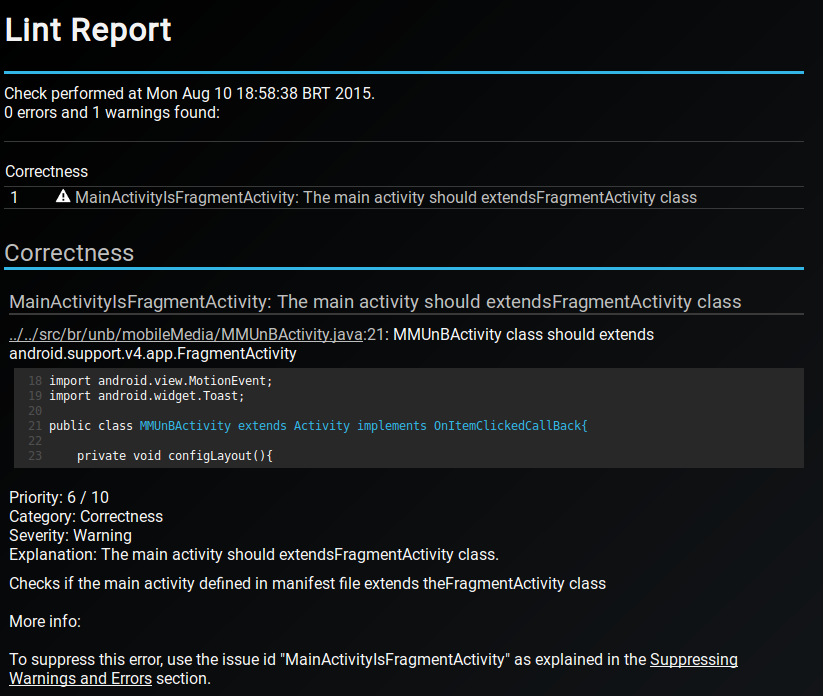
\includegraphics[width=15cm]{img/activity_deve_ser_container.png}
    \caption{Aviso de que a activity deve herdar de FragmentActivity}
    \label{activity_deve_ser_container}
\end{figure}

Para resolver esse problema, basta seguir a orientação apresentada no relatório
e fazer com que a activity {\it MMUnBActivity} herde da classe
{\it android.support.v4.app.FragmentActivity}, conforme apresentado na figura
\ref{herda_FragmentActivity}

\begin{figure}[h]
    \centering
    
\includegraphics[width=15cm]{img/heranca_FragmentActivity.png}
    \caption{Activity corretamente extendendo de FragmentActivity}
    \label{herda_FragmentActivity}
\end{figure}

Além de ser um container de fragmentos, é também necessário que a activity seja,
de fato, composto por eles. Existem duas formas de fazer essa composição:
declarando o fragmento no arquivo XML de layout da activity ou programaticamente
adicionando o fragmento na activity. Nessa proposta inicial, foi considerada
somente a forma programatica.

Para fazer a inclusão de forma programatica, um determinado conjunto de métodos
deverá ser executado: {\it getSupportFragmentManager} para obter um objeto {\it
FragmentManager}. Então chamar {\it beginTransaction()} para criar um {\it
FragmentTransaction} e, por fim, {\it add()} para adicionar o fragmento. Também
deve ser executado {\it commit()} quando realizamos múltiplas transações de 
fragmentos com o mesmo {\it FragmentTransaction}. Um exemplo disso pode ser visto
na figura \ref{adicao_fragmento}, que apresenta o método {\it onCreate} da classe
{\it MMUnBActivity}.

\begin{figure}[h]
    \centering
    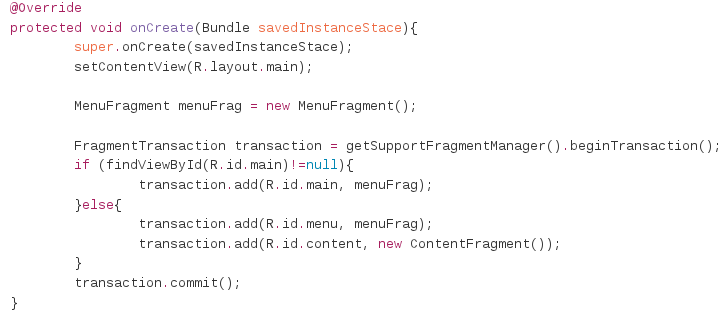
\includegraphics[width=15cm]{img/add_fragment.png}
    \caption{Adicionando framentos de forma programática}
    \label{adicao_fragmento}
\end{figure}

Embora vários métodos sejam utilizados, nessa abordagem verificamos apenas se o
o método {\it beginTransaction()} do {\it FragmentManager} é chamado a partir do
{\it onCreate()} da activity, inclusive de forma recursiva. Empiricamente,
acreditamos que se esse método está sendo chamado, os demais necessários para a
adição do correta do(s) fragmento(s) a activity também estão. Essa análise é feita
para cada classe da aplicação que estende {\it FragmentActivity}.

\section{Uso da API ActionBar}

A partir do Android 3.0 (API Level 11), a action bar é incluida em todas as
activities que usam o tema Theme.Holo (ou um dos seus descendentes), e que é o
tema padrão quando os atributos {\it targetSdkVersion} ou {\it minSdkVersion}
estão definidos para "11" ou maior.

Para versões anteriores, é possível utilizar o pacote de compatibilidade V7.
Nesse caso, serão necessários dois passos adicionais:

\begin{itemize}
  \item{A activity deve estender ActionBarActivity;}
  \item{A activity deve usar um tema da família Theme.AppCompat, como o
  Theme.AppCompat.Light}
\end{itemize}

Para o primeiro item, a verificação e feita de forma semelhante ao apresentação
na seção \ref{uso_fragments}. Inclusive ActionBarActivity herda de FragmentActivity.
Assim, essa verificação não inválida a descrita naquela seção.

Quando uma activity atende ao primeiro item, o segundo é analisado. Para tal,
é recuperado do arquivo de manifesto o elemento referente à activity e então
o atributo {\it theme} é comparado com {\it Theme.AppCompat.Light}, reportando
um erro caso seja diferente.


\chapter{Conclusão}
Escrever a conclusão do trabalho...



% ==============================================================================
\nocite*
\bibliographystyle{apalike}
%\bibliographystyle{abnt-alf}
\bibliography{biblio}
\begin{landscape}
\appendix
\chapter{Checks predefinidos do Android Lint relacionados a padrões e variabilidades}

\begin{longtable}{p{30mm}|p{180mm}|p{25mm}}
%\caption[Feasible triples for a highly variable Grid]{Feasible triples for highly variable Grid, MLMMH.} \label{grid_mlmmh} \\

\hline \multicolumn{1}{|c|}{\textbf{Check}} & \multicolumn{1}{c|}{\textbf{Descrição}} & \multicolumn{1}{c|}{\textbf{Variabilidade}} \\ \hline 
\endfirsthead

\multicolumn{3}{c}%
{{\bfseries \tablename\ \thetable{} -- continuação da página anterior}} \\
\hline \multicolumn{1}{|c|}{\textbf{Check}} &
\multicolumn{1}{c|}{\textbf{Descrição}} &
\multicolumn{1}{c|}{\textbf{Variabilidade}} \\ \hline 
\endhead

\hline \multicolumn{3}{|r|}{{Continua na próxima página}} \\ \hline
\endfoot

\hline \hline
\endlastfoot

\hline                               
UnusedAttribute & 
This check finds attributes set in XML files that were introduced in a version
newer than the oldest version targeted by your application (with the the minSdkVersion
attribute). This is not an error; the application will simply ignore the attribute.
However, if the attribute is important to the appearance of functionality of your
application, you should consider finding an alternative way to achieve the same
result with only available attributes, and then you can optionally create a copy
of the layout in a layout-vNN folder which will be used on API NN or higher where
you can take advantage of the newer attribute. Note: This check does not only apply
to attributes. For example, some tags can be unused too, such as the new <tag> element
in layouts introduced in API 21.
& Diferentes versões da API \\

Back button & According to the Android Design Guide, "Other platforms use an explicit
back button with label to allow the user to navigate up the application's hierarchy.
Instead, Android uses the main action bar's app icon for hierarchical navigation
and the navigation bar's back button for temporal navigation." This check is not
very sophisticated (it just looks for buttons with the label "Back"), so it is
disabled by default to not trigger on common scenarios like pairs of Back/Next
buttons to paginate through screens. http://developer.android.com/design/patterns/pure-android.html
& Padrão de Design \\

Button order & According to the Android Design Guide, "Action buttons are typically
Cancel and/or OK, with OK indicating the preferred or most likely action. However,
if the options consist of specific actions such as Close or Wait rather than a
confirmation or cancellation of the action described in the content, then all the
buttons should be active verbs. As a rule, the dismissive action of a dialog is
always on the left whereas the affirmative actions are on the right." This check
looks for button bars and buttons which look like cancel buttons, and makes sure
that these are on the left. http://developer.android.com/design/building-blocks/dialogs.html
& Padrão de Design \\

Button should be borderless & Button bars typically use a borderless style for
the buttons. Set the style="?android:attr/buttonBarButtonStyle" attribute on each
of the buttons, and set style="?android:attr/buttonBarStyle" on the parent layout
http://developer.android.com/design/building-blocks/buttons.html
& Padrão de Design \\

Byte order mark inside files & Lint will flag any byte-order-mark (BOM) characters
it finds in the middle of a file. Since we expect files to be encoded with UTF-8
(see the EnforceUTF8 issue), the BOM characters are not necessary, and they are
not handled correctly by all tools. For example, if you have a BOM as part of a
resource name in one particular translation, that name will not be considered
identical to the base resource's name and the translation will not be used.
http://en.wikipedia.org/wiki/Byte\_order\_mark
& No exemplo dado, pode ter influencia na variabilidade de idiomas\\
 
Calling new methods on older versions
&This check scans through all the Android API calls in the application and warns about any calls that are not available on all versions targeted by this application (according to its minimum SDK attribute in the manifest). If you really want to use this API and don't need to support older devices just set the minSdkVersion in your build.gradle or AndroidManifest.xml files. If your code is deliberately accessing newer APIs, and you have ensured (e.g. with conditional execution) that this code will only ever be called on a supported platform, then you can annotate your class or method with the @TargetApi annotation specifying the local minimum SDK to apply, such as @TargetApi(11), such that this check considers 11 rather than your manifest file's minimum SDK as the required API level. If you are deliberately setting android: attributes in style definitions, make sure you place this in a values-vNN folder in order to avoid running into runtime conflicts on certain devices where manufacturers have added custom attributes whose ids conflict with the new ones on later platforms. Similarly, you can use tools:targetApi="11" in an XML file to indicate that the element will only be inflated in an adequate context.
&Diferentes versões da API\\

Cancel/OK dialog button capitalization
&The standard capitalization for OK/Cancel dialogs is "OK" and "Cancel". To ensure that your dialogs use the standard strings, you can use the resource strings @android:string/ok and @android:string/cancel.
&Padrao de Design\\

Clashing PNG and 9-PNG files
&If you accidentally name two separate resources file.png and file.9.png, the image file and the nine patch file will both map to the same drawable resource, @drawable/file, which is probably not what was intended.
&"Imagens que podem ser utilizadas em telas de tamanhos/resoluções diferente
(um referencia: http://www.thiengo.com.br/9-patch-no-android-mantendo-a-qualidade-de-imagens-de-background)"\\

Class is not registered in the manifest
&Activities, services and content providers should be registered in the AndroidManifest.xml file using <activity>, <service> and <provider> tags. If your activity is simply a parent class intended to be subclassed by other "real" activities, make it an abstract class. http://developer.android.com/guide/topics/manifest/manifest-intro.html
&Útil quando “activity is simply a parent class intended to be subclassed by other "real" activities” e cada subclasse será implementação de uma variante\\

Custom views in libraries should use res-auto-namespace
&When using a custom view with custom attributes in a library project, the layout must use the special namespace http://schemas.android.com/apk/res-auto instead of a URI which includes the library project's own package. This will be used to automatically adjust the namespace of the attributes when the library resources are merged into the application project.
&Se o núcleo de uma LPS for definido como um “library project” isso será ser útil\\

Deprecated Gradle Construct
&This detector looks for deprecated Gradle constructs which currently work but will likely stop working in a future update.
&Variabilidade de plataforma, mas em tempo de projeto, não de execução\\

Duplicated icons under different names
&If an icon is repeated under different names, you can consolidate and just use one of the icons and delete the others to make your application smaller. However, duplicated icons usually are not intentional and can sometimes point to icons that were accidentally overwritten or accidentally not updated.
&Pode influenciar em dispositivos com pouco espaço\\

Dynamic text should probably be selectable
&Dynamic text should probably be selectable If a <TextView> is used to display data, the user might want to copy that data and paste it elsewhere. To allow this, the <TextView> should specify android:textIsSelectable="true". This lint check looks for TextViews which are likely to be displaying data: views whose text is set dynamically. This value will be ignored on platforms older than API 11, so it is okay to set it regardless of your minSdkVersion.
&Relacionado com versões diferentes da API\\

Encoding used in resource files is not UTF-8
&XML supports encoding in a wide variety of character sets. However, not all tools handle the XML encoding attribute correctly, and nearly all Android apps use UTF-8, so by using UTF-8 you can protect yourself against subtle bugs when using non-ASCII characters. In particular, the Android Gradle build system will merge resource XML files assuming the resource files are using UTF-8 encoding.
&Variabilidade de plataforma, mas em tempo de projeto, não de execução\\

Extra translation
&If a string appears in a specific language translation file, but there is no corresponding string in the default locale, then this string is probably unused. (It's technically possible that your application is only intended to run in a specific locale, but it's still a good idea to provide a fallback.). Note that these strings can lead to crashes if the string is looked up on any locale not providing a translation, so it's important to clean them up.
&Variabilidade de idioma\\

Formatting argument types incomplete or inconsistent
&When a formatted string takes arguments, it usually needs to reference the same arguments in all translations (or all arguments if there are no translations. There are cases where this is not the case, so this issue is a warning rather than an error by default. However, this usually happens when a language is not translated or updated correctly.
&Variabilidade de idioma\\

Fragment not instantiatable
&From the Fragment documentation: Every fragment must have an empty constructor, so it can be instantiated when restoring its activity's state. It is strongly recommended that subclasses do not have other constructors with parameters, since these constructors will not be called when the fragment is re-instantiated; instead, arguments can be supplied by the caller with setArguments(Bundle) and later retrieved by the Fragment with getArguments(). http://developer.android.com/reference/android/app/Fragment.html\#Fragment()
&Relacionado a tamanho de telas quando o framento é usado pra trata esse tipo de variabilidade\\

Fragments should specify an id or tag
&If you do not specify an android:id or an android:tag attribute on a <fragment> element, then if the activity is restarted (for example for an orientation rotation) you may lose state. From the fragment documentation: "Each fragment requires a unique identifier that the system can use to restore the fragment if the activity is restarted (and which you can use to capture the fragment to perform transactions, such as remove it). * Supply the android:id attribute with a unique ID. * Supply the android:tag attribute with a unique string. If you provide neither of the previous two, the system uses the ID of the container view. http://developer.android.com/guide/components/fragments.html
&Relacionado a tamanho de telas quando o framento é usado pra trata esse tipo de variabilidade\\

Gradle Dynamic Version
&Using + in dependencies lets you automatically pick up the latest available version rather than a specific, named version. However, this is not recommended; your builds are not repeatable; you may have tested with a slightly different version than what the build server used. (Using a dynamic version as the major version number is more problematic than using it in the minor version position.)
&Variabilidade de plataforma, mas em tempo de projeto, não de execução\\

Gradle IDE Support Issues
&Gradle is highly flexible, and there are things you can do in Gradle files which can make it hard or impossible for IDEs to properly handle the project. This lint check looks for constructs that potentially break IDE support.
&Variabilidade de plataforma, mas em tempo de projeto, não de execução\\

Gradle Path Issues
&Gradle build scripts are meant to be cross platform, so file paths use Unix-style path separators (a forward slash) rather than Windows path separators (a backslash). Similarly, to keep projects portable and repeatable, avoid using absolute paths on the system; keep files within the project instead. To share code between projects, consider creating an android-library and an AAR dependency
&Variabilidade de plataforma, mas em tempo de projeto, não de execução\\

Hardcoded Package in Namespace
&In Gradle projects, the actual package used in the final APK can vary; for you can add a .debug package suffix in one version and not the other. Therefore, you should not hardcode the application package in the resource; instead, use the special namespace http://schemas.android.com/apk/res-auto which will cause the tools to figure out the right namespace for the resource regardless of the actual package used during the build.
&Util para gerar versões diferentes da mesma app\\

Hardcoded reference to /sdcard
&Your code should not reference the /sdcard path directly; instead use Environment.getExternalStorageDirectory().getPath(). Similarly, do not reference the /data/data/ path directly; it can vary in multi-user scenarios. Instead, use Context.getFilesDir().getPath(). http://developer.android.com/guide/topics/data/data-storage.html\#filesExternal
&Aparelhos pode ter ou não certos recursos (sdcard, no caso)\\

HashMap can be replaced with SparseArray
&For maps where the keys are of type integer, it's typically more efficient to use the Android SparseArray API. This check identifies scenarios where you might want to consider using SparseArray instead of HashMap for better performance. This is particularly useful when the value types are primitives like ints, where you can use SparseIntArray and avoid auto-boxing the values from int to Integer. If you need to construct a HashMap because you need to call an API outside of your control which requires a Map, you can suppress this warning using for example the @SuppressLint annotation.
&Variantes de implementaçao de “maps”, mas com efeito somente em tempo de projeto, an não ser pela performance de execução\\

Icon appears in both -nodpi and dpi folders
&Bitmaps that appear in drawable-nodpi folders will not be scaled by the Android framework. If a drawable resource of the same name appears both in a -nodpi folder as well as a dpi folder such as drawable-hdpi, then the behavior is ambiguous and probably not intentional. Delete one or the other, or use different names for the icons.
&Telas de tamanhos diferentes\\

Icon colors do not follow the recommended visual style
&Notification icons and Action Bar icons should only white and shades of gray. See the Android Design Guide for more details. Note that the way Lint decides whether an icon is an action bar icon or a notification icon is based on the filename prefix: ic\_menu\_ for action bar icons, ic\_stat\_ for notification icons etc. These correspond to the naming conventions documented in http://developer.android.com/guide/practices/ui\_guidelines/icon\_design.html http://developer.android.com/design/style/iconography.html
&Padrao de Design\\

Icon densities validation
&Icons will look best if a custom version is provided for each of the major screen density classes (low, medium, high, extra high). This lint check identifies icons which do not have complete coverage across the densities. Low density is not really used much anymore, so this check ignores the ldpi density. To force lint to include it, set the environment variable ANDROID\_LINT\_INCLUDE\_LDPI=true. For more information on current density usage, see http://developer.android.com/resources/dashboard/screens.html
&Telas diferentes\\

Icon density-independent size validation
&Checks the all icons which are provided in multiple densities, all compute to roughly the same density-independent pixel (dip) size. This catches errors where images are either placed in the wrong folder, or icons are changed to new sizes but some folders are forgotten.
&Telas diferentes\\

Icon density-independent size validation
&Checks the all icons which are provided in multiple densities, all compute to roughly the same density-independent pixel (dip) size. This catches errors where images are either placed in the wrong folder, or icons are changed to new sizes but some folders are forgotten
&Telas diferentes\\

Icon has incorrect size
&There are predefined sizes (for each density) for launcher icons. You should follow these conventions to make sure your icons fit in with the overall look of the platform.
&Telas diferentes\\

Identical bitmaps across various configurations
&If an icon is provided under different configuration parameters such as drawable-hdpi or -v11, they should typically be different. This detector catches cases where the same icon is provided in different configuration folder which is usually not intentional
&Telas diferentes\\

Image defined in density-independent drawable folder
&The res/drawable folder is intended for density-independent graphics such as shapes defined in XML. For bitmaps, move it to drawable-mdpi and consider providing higher and lower resolution versions in drawable-ldpi, drawable-hdpi and drawable-xhdpi. If the icon really is density independent (for example a solid color) you can place it in drawable-nodpi
&Telas diferentes\\

Implied locale in date format
&"Almost all callers should use getDateInstance(), getDateTimeInstance(), or getTimeInstance() to get a ready-made instance of SimpleDateFormat suitable for the user's locale. The main reason you'd create an instance this class directly is because you need to format/parse a specific machine-readable format, in which case you almost certainly want to explicitly ask for US to
ensure that you get ASCII digits (rather than, say, Arabic digits).
Therefore, you should either use the form of the SimpleDateFormat constructor where you pass in an explicit locale, such as Locale.US, or use one of the get instance methods, or suppress this error if really know what you are doing"
&Internacionalização\\

Implied Quantities
&Plural strings should generally include a \%s or \%d formatting argument. In locales like English, the one quantity only applies to a single value, 1, but that's not true everywhere. For example, in Slovene, the one quantity will apply to 1, 101, 201, 301, and so on. Similarly, there are locales where multiple values match the zero and two quantities.
In these locales, it is usually an error to have a message which does not include a formatting argument (such as '\%d'), since it will not be clear from the grammar what quantity the quantity string is describing
&Internacionalização\\

Incomplete translation
&If an application has more than one locale, then all the strings declared in one language should also be translated in all other languages.  If the string should not be translated, you can add the attribute translatable="false" on the <string> element, or you can define all your non-translatable strings in a resource file called donottranslate.xml. Or, you can ignore the issue with a tools:ignore="MissingTranslation" attribute.  By default this detector allows regions of a language to just provide a subset of the strings and fall back to the standard language strings. You can require all regions to provide a full translation by setting the environment variable ANDROID\_LINT\_COMPLETE\_REGIONS.  You can tell lint (and other tools) which language is the default language in your res/values/ folder by specifying tools:locale="languageCode" for the root <resources> element in your resource file. (The tools prefix refers to the namespace declaration http://schemas.android.com/tools.)
&Variabilidade de Idiomas\\

Inefficient layout weight
&When only a single widget in a LinearLayout defines a weight, it is more efficient to assign a width/height of 0dp to it since it will absorb all the remaining space anyway. With a declared width/height of 0dp it does not have to measure its own size first.
&Telas diferentes\\

Minimum SDK and target SDK attributes not defined
&The manifest should contain a <uses-sdk> element which defines the minimum API Level required for the application to run, as well as the target version (the highest API level you have tested the version for.)
&SDK version\\

Missing commit() calls
&After creating a FragmentTransaction, you typically need to commit it as well
&Uso de fragmentos\\

Missing density folder
&Icons will look best if a custom version is provided for each of the major screen density classes (low, medium, high, extra-high, extra-extra-high). This lint check identifies folders which are missing, such as drawable-hdpi. Low density is not really used much anymore, so this check ignores the ldpi density. To force lint to include it, set the environment variable ANDROID\_LINT\_INCLUDE\_LDPI=true. For more information on current density usage, see http://developer.android.com/resources/dashboard/screens.html
&Telas Diferentes\\

Missing explicit orientation
&The default orientation of a LinearLayout is horizontal. It's pretty easy to believe that the layout is vertical, add multiple children to it, and wonder why only the first child is visible (when the subsequent children are off screen to the right). This lint rule helps pinpoint this issue by warning whenever a LinearLayout is used with an implicit orientation and multiple children.  It also checks for empty LinearLayouts without an orientation attribute that also defines an id attribute. This catches the scenarios where children will be added to the LinearLayout dynamically.
&Telas Diferentes
 
%\end{tabular}
\end{longtable}

\end{landscape}

% ==============================================================================
\end{document}
